% Provenance (never printed): lycee terminale S SVT "Les climats de la Terre"
% and the 2019 enseignement scientifique ("Le climat de la Terre": forcing,
% feedbacks, the IPCC assessments, scenarios), union; physical science only,
% as the user ruled (2026-10-22). See sources/outline_sources.md. Pilot
% chapter, 2026-10-22. Every figure about the climate system is an IPCC AR6
% WG1 statement (ledger ipcc:*) or computed from a dataset in
% figdata/grade-12/climate_records.py.
\chapter{El cambio climático: observaciones, causas y proyecciones}\label{ch:g12:climate-change}

En lo alto de la ladera norte del Mauna Loa, un volcán en medio del
océano Pacífico, un grupo de edificios blancos se alza sobre la lava desnuda,
a \qty{3397}{m} sobre el nivel del mar. Allí arriba, por encima de la capa de aire contaminada por
la isla de abajo y a miles de kilómetros de cualquier gran ciudad, el aire
es casi tan limpio y está casi tan bien mezclado como la atmósfera de todo el planeta. Desde
marzo de 1958, su dióxido de carbono se mide casi sin interrupción.
El registro empezó como el proyecto de un químico; se ha convertido en la
curva más famosa de las ciencias de la Tierra. Este capítulo lee esa curva y los demás registros
del clima, explica cómo un cambio en el aire modifica el \omterm{def:g10:earth-energy-budget:energy-budget}{balance energético}
del planeta y cómo deciden los científicos qué causó el calentamiento que observan,
y presenta lo que proyectan para las próximas décadas.
% ledger: noaa:mlo-site, noaa:keeling-1958

\begin{omfigure}
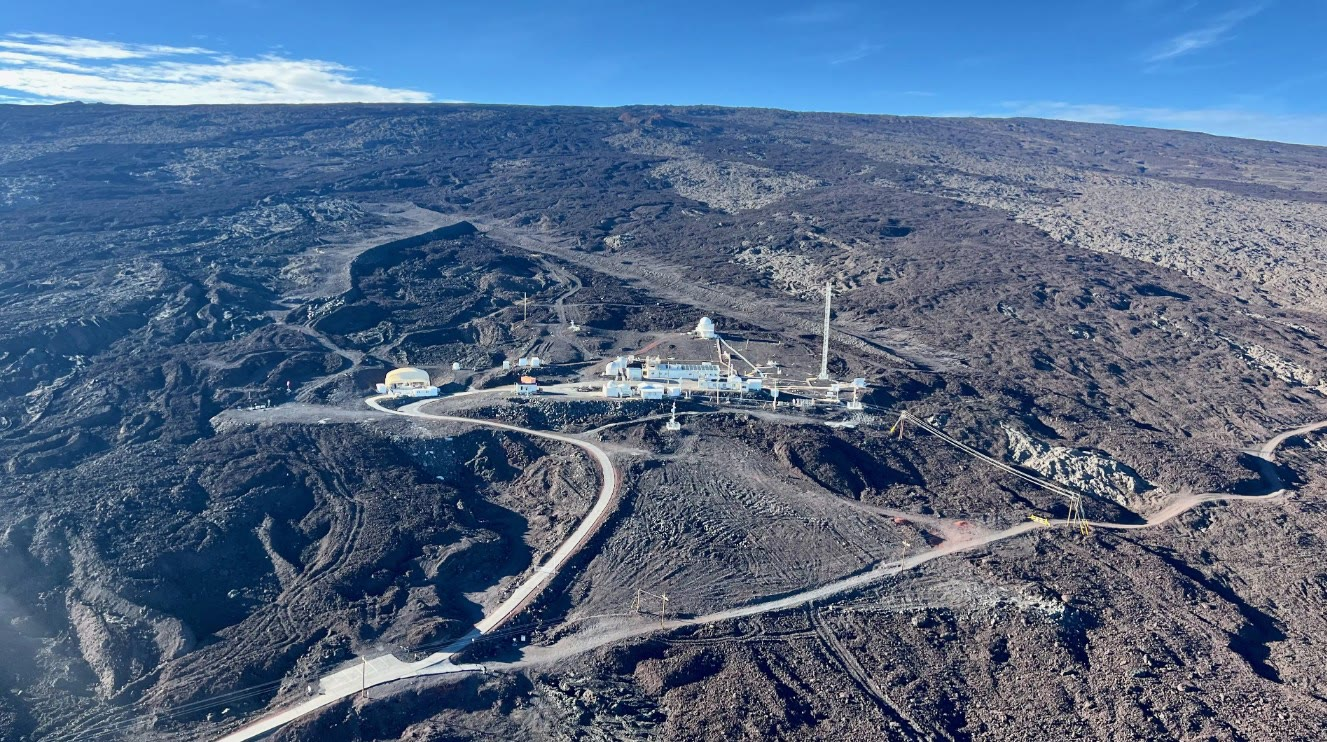
\includegraphics[width=0.78\linewidth]{images/book2/g12-noaa-mauna-loa-observatory.jpg}

{\small El observatorio de Mauna Loa, Hawái, sobre antiguas coladas de lava en lo alto de la
ladera norte del volcán. Fotografía: Brian Vasel, NOAA (dominio público).}
\end{omfigure}

\begin{recall}
La Tierra recibe energía del Sol en forma de luz y pierde en promedio la misma cantidad
hacia el espacio en forma de radiación infrarroja; la fracción de la luz solar reflejada
es el \omterm{def:g10:earth-energy-budget:albedo}{albedo} (el \cref{ch:g10:earth-energy-budget}). Los gases de efecto invernadero ---el vapor
de agua, el dióxido de carbono, el metano--- absorben parte del infrarrojo que emite la
superficie y devuelven una parte hacia abajo; este efecto invernadero mantiene
la superficie mucho más caliente de lo que estaría sin él (los libros de química;
Libro 1, año 9). Los \omterm{def:g12:past-climates:ice-core}{testigos de hielo} guardan burbujas de aire antiguo y registran los
\omterm{def:g12:past-climates:glacial-cycle}{ciclos glaciales} de los últimos 800\,000 años (el \cref{ch:g12:past-climates}).
\end{recall}

\section{Los registros}

\begin{omfigure}
\begin{tikzpicture}
\begin{axis}[omrecord, width=0.92\linewidth, height=6.2cm, xmin=1957, xmax=2028,
  ymin=305, ymax=440, xlabel={año}, ylabel={dióxido de carbono (ppm)},
  xtick={1960,1970,...,2020}, /pgf/number format/1000 sep={}]
\addplot[omDef!85!black, line width=0.5pt] table[x=decimal_year, y=co2_ppm] {figdata/out/grade-12-climate_records-co2.dat};
\addplot[only marks, mark=*, mark size=0.9pt, omThm!85!black] table[x=year, y=co2_ppm] {figdata/out/grade-12-climate_records-co2annual.dat};
\end{axis}
\end{tikzpicture}

{\small El contenido de dióxido de carbono del aire en Mauna Loa: medias mensuales
(línea) y medias anuales (puntos), en partes por millón (ppm) de aire seco.
Datos: NOAA Global Monitoring Laboratory y Scripps Institution of
Oceanography.}
\end{omfigure}

\begin{proposition}[El registro del dióxido de carbono]\label{prop:g12:climate-change:co2}
% ledger: data:co2-mlo (all numbers computed in figdata/grade-12/climate_records.py)
En Mauna Loa, la concentración media anual de dióxido de carbono pasó de
\qty{316.0}{ppm} en 1959 a \qty{427.4}{ppm} en 2025, y el aumento se
acelera: la concentración creció unos \qty{0.9}{ppm} al año en
los años sesenta y unos \qty{2.6}{ppm} al año entre 2015 y 2025. Cada
año, la concentración oscila además unos \qty{7}{ppm}: es máxima en
mayo y mínima en septiembre.
\end{proposition}

\begin{remark}[Por qué la curva tiene dientes]\label{rem:g12:climate-change:teeth}
La oscilación anual es la respiración de la vegetación del hemisferio
norte, donde está la mayoría de las plantas terrestres. En primavera y verano, las plantas captan
más dióxido de carbono por fotosíntesis del que liberan ellas y el suelo;
en otoño e invierno ganan la descomposición y la respiración. El aumento de un año
a otro es otra historia: es el carbono de los combustibles fósiles y de los bosques
talados que se acumula en el aire.
\end{remark}

\begin{proposition}[Más alto que en al menos dos millones de años]\label{prop:g12:climate-change:icecore}
% ledger: data:co2-bereiter (173.7 and 298.6 ppm computed), ipcc:co2-2myr (high confidence)
En los últimos 800\,000 años, las burbujas de aire del hielo antártico registran
concentraciones de dióxido de carbono de entre unos \qty{174}{ppm}, en los \omterm{def:g12:past-climates:glacial-cycle}{periodos
glaciales} más fríos, y \qty{299}{ppm}, en los \omterm{def:g12:past-climates:glacial-cycle}{interglaciales} más cálidos. El valor
actual está más de \qty{100}{ppm} por encima del más alto de ellos. Las
evaluaciones afirman que la concentración de 2019 era más alta que en ningún otro momento
de al menos los últimos dos millones de años (\emph{confianza alta}).
\end{proposition}

\begin{omfigure}
\begin{tikzpicture}
\begin{axis}[omrecord, omage, width=0.92\linewidth, height=5.2cm, xmin=0, xmax=810,
  ymin=150, ymax=490, xlabel={miles de años antes de 1950},
  ylabel={dióxido de carbono (ppm)}, xtick={0,100,...,800}]
\addplot[omDef!85!black, line width=0.6pt] table[x=age_kyr, y=co2_ppm] {figdata/out/grade-12-climate_records-icecore.dat};
\draw[omThm, densely dashed, line width=0.8pt] (axis cs:810,427.35) -- (axis cs:0,427.35);
\node[font=\footnotesize, text=omThm!85!black, anchor=south west] at (axis cs:780,433) {media anual en Mauna Loa en 2025};
\end{axis}
\end{tikzpicture}

{\small El dióxido de carbono del hielo antártico a lo largo de 800\,000 años: los \omterm{def:g12:past-climates:glacial-cycle}{ciclos
glaciales} lo hacen variar entre unos 180 y \qty{300}{ppm}. El fino pico del
extremo derecho es el hielo más joven, que registra el comienzo del aumento
actual, hasta el año 2001. Datos: Bereiter y otros (2015), NOAA
Paleoclimatology.}
% the youngest sample of the composite: age -51 yr BP (2001), 368.02 ppm (data/derived/co2-icecore.csv)
\end{omfigure}

\begin{omfigure}
\begin{tikzpicture}
\begin{axis}[omrecord, width=0.92\linewidth, height=5.6cm, xmin=1878, xmax=2027,
  ymin=-0.6, ymax=1.45, xlabel={año},
  ylabel={anomalía de temperatura (\unit{\degreeCelsius})},
  xtick={1880,1900,...,2020}, /pgf/number format/1000 sep={},
  legend style={at={(0.03,0.96)}, anchor=north west, font=\footnotesize, draw=black!30}]
\addplot[omDef!70, line width=0.5pt, mark=*, mark size=0.6pt] table[x=year, y=anomaly] {figdata/out/grade-12-climate_records-temp.dat};
\addlegendentry{media anual}
\addplot[omThm!85!black, line width=1.3pt, unbounded coords=jump] table[x=year, y=mean11] {figdata/out/grade-12-climate_records-temp.dat};
\addlegendentry{media de 11 años}
\end{axis}
\end{tikzpicture}

{\small Temperatura media global en superficie, como diferencia respecto a su media
de 1951--1980. Datos: NASA GISS Surface Temperature Analysis (GISTEMP v4).}
\end{omfigure}

\begin{proposition}[El calentamiento global observado]\label{prop:g12:climate-change:warming}
% ledger: ipcc:gsat-2011-2020, ipcc:decades
Cada una de las cuatro últimas décadas ha sido más cálida que cualquier década anterior
desde 1850. La temperatura global en superficie de 2011--2020 fue \qty{1.09}{\degreeCelsius}
más alta que la de 1850--1900 (muy probablemente entre 0.95 y
\qty{1.20}{\degreeCelsius}), con más calentamiento sobre los continentes
(\qty{1.59}{\degreeCelsius}) que sobre el océano (\qty{0.88}{\degreeCelsius}).
\end{proposition}

\begin{proposition}[El nivel del mar sube cada vez más deprisa]\label{prop:g12:climate-change:sea}
% ledger: ipcc:sea-level-obs, data:gmsl-lsa (3.2 mm/yr trend computed)
El nivel medio global del mar subió unos \qty{0.20}{m} entre 1901 y 2018.
El ritmo fue de unos \qty{1.3}{mm} al año de 1901 a 1971,
\qty{1.9}{mm} al año de 1971 a 2006 y \qty{3.7}{mm} al año de
2006 a 2018 (\emph{confianza alta}). Los satélites, que miden la altura de
la superficie del mar desde 1993, dan una media de \qty{3.2}{mm} al año en
1993--2025. El mar sube porque el océano, al calentarse, se dilata y porque
los glaciares y los inlandsis le ceden hielo.
\end{proposition}

\begin{omfigure}
\begin{tikzpicture}
\begin{axis}[omrecord, width=0.86\linewidth, height=5cm, xmin=1992, xmax=2026,
  ymin=-35, ymax=95, xlabel={año}, ylabel={nivel del mar (mm)},
  /pgf/number format/1000 sep={}, xtick={1995,2000,...,2025}]
\addplot[omDef!85!black, line width=0.5pt] table[x=decimal_year, y=gmsl_mm] {figdata/out/grade-12-climate_records-sea.dat};
\end{axis}
\end{tikzpicture}

{\small Nivel medio global del mar medido desde el espacio, aproximadamente cada diez días
(sin la señal estacional), respecto a un cero arbitrario. Los datos de altimetría
proceden del NOAA Laboratory for Satellite Altimetry.}
\end{omfigure}

\begin{dated}{2025}
% ledger: data:co2-mlo, data:gistemp (values read from the datasets as fetched 2026-10-22)
La concentración media anual de dióxido de carbono en Mauna Loa en 2025 fue de
\qty{427.35}{ppm}. En el registro de temperatura de la NASA, el año más cálido hasta ahora
fue 2024, con \qty{1.28}{\degreeCelsius} por encima de la media de 1951--1980.
\end{dated}

\section{El forzamiento radiativo}

\begin{definition}[Forzamiento radiativo]\label{def:g12:climate-change:forcing}
El \emph{forzamiento radiativo}\index{forzamiento radiativo} de un cambio en el
sistema climático ---más gas de efecto invernadero, más partículas de aerosol, un Sol
más brillante--- es el cambio que provoca en el flujo neto de energía que entra en el
sistema climático en lo alto de la atmósfera, antes de que la temperatura de la superficie
haya tenido tiempo de responder. Se mide en vatios por metro cuadrado
(\unit{W/m^2}) de superficie terrestre. Un forzamiento positivo hace que el planeta
gane energía y se caliente; uno negativo hace que pierda energía y se enfríe.
\end{definition}

\begin{remark}[Forzamiento efectivo]\label{rem:g12:climate-change:effective}
Las evaluaciones usan el \omterm{def:g12:climate-change:forcing}{forzamiento radiativo} \emph{efectivo}, que tiene en cuenta además
los ajustes rápidos de la atmósfera (de sus nubes, por ejemplo)
que se producen antes de que la superficie se caliente. Todos los \omterm{def:g12:climate-change:forcing}{forzamientos} de este capítulo son
\omterm{def:g12:climate-change:forcing}{forzamientos} efectivos.
\end{remark}

\begin{proposition}[El forzamiento desde 1750]\label{prop:g12:climate-change:forcing}
% ledger: ipcc:erf-total, ipcc:erf-agents
Las actividades humanas han producido un \omterm{def:g12:climate-change:forcing}{forzamiento radiativo} total de
\qty{2.72}{W/m^2} en 2019 respecto a 1750 (muy probablemente entre 1.96 y
\qty{3.48}{W/m^2}). Los gases de efecto invernadero aportan un \omterm{def:g12:climate-change:forcing}{forzamiento} positivo, encabezado
por el dióxido de carbono (\qty{2.16}{W/m^2}); las partículas de aerosol, que reflejan la
luz solar y hacen más brillantes las nubes, aportan uno negativo (unos
\qty{-1.06}{W/m^2} en total). El cambio del brillo del Sol en el
mismo periodo aporta solo \qty{0.01}{W/m^2}.
\end{proposition}

\begin{omfigure}
% ledger: ipcc:erf-agents, ipcc:erf-total (central values and 5-95 % ranges of AR6 Table 7.8)
\begin{tikzpicture}
\begin{axis}[xbar, width=0.8\linewidth, height=7.2cm, xmin=-1.8, xmax=3.7,
  ytick={1,...,10}, yticklabels={total (humano), solar, uso del suelo,
  aerosoles--nubes, aerosoles--radiación, ozono, gases halogenados, óxido nitroso,
  metano, dióxido de carbono}, y tick label style={font=\small},
  tick label style={font=\small}, xlabel={forzamiento radiativo efectivo, 1750--2019 (\unit{W/m^2})},
  label style={font=\small}, bar width=6pt, bar shift=0pt, axis x line=bottom, axis y line=left,
  axis line style={-}, enlarge y limits=0.07, xmajorgrids,
  grid style={gray!22, line width=0.3pt}, extra x ticks={0},
  extra x tick style={grid style={black!60, line width=0.5pt}}]
\addplot[fill=omThm!55, draw=omThm!80!black, error bars/.cd, x dir=both, x explicit,
  error bar style={black!70}] coordinates {
  (2.16,10) += (0.25,0) -= (0.26,0)
  (0.54,9) += (0.11,0) -= (0.11,0)
  (0.21,8) += (0.03,0) -= (0.03,0)
  (0.41,7) += (0.08,0) -= (0.08,0)
  (0.47,6) += (0.24,0) -= (0.23,0)
  (2.72,1) += (0.76,0) -= (0.76,0)
  (0.01,2) += (0.07,0) -= (0.07,0)};
\addplot[fill=omDef!55, draw=omDef!80!black, error bars/.cd, x dir=both, x explicit,
  error bar style={black!70}] coordinates {
  (-0.22,5) += (0.26,0) -= (0.25,0)
  (-0.84,4) += (0.59,0) -= (0.61,0)
  (-0.20,3) += (0.10,0) -= (0.10,0)};
\end{axis}
\end{tikzpicture}

{\small Los principales \omterm{def:g12:climate-change:forcing}{forzamientos radiativos} efectivos de 1750 a 2019, con sus
intervalos muy probables (bigotes). Valores: IPCC, Sexto Informe de Evaluación, Grupo
de Trabajo~I, tabla 7.8.}
\end{omfigure}

\begin{proposition}[Dióxido de carbono: cada duplicación añade el mismo forzamiento]\label{prop:g12:climate-change:log}
% ledger: ipcc:erf-2xco2, ipcc:log-co2
En buena aproximación, el \omterm{def:g12:climate-change:forcing}{forzamiento} del dióxido de carbono crece con el
\emph{logaritmo} de su concentración: cada duplicación añade el mismo \omterm{def:g12:climate-change:forcing}{forzamiento},
$F_{2\times} = \qty{3.93}{W/m^2}$ para una duplicación a partir de la concentración de
1750, $C_0 = \qty{278}{ppm}$. El \omterm{def:g12:climate-change:forcing}{forzamiento} de una concentración $C$ es entonces
\[
  F = F_{2\times}\,\frac{\ln (C/C_0)}{\ln 2}.
\]
\end{proposition}

\begin{example}[Comprobar la ley con la evaluación]\label{ex:g12:climate-change:check}
% ledger: ipcc:erf-2xco2, ipcc:erf-agents
En 2019 la concentración era de \qty{410}{ppm}. La ley da
$F = 3.93 \times \ln(410/278)/\ln 2 = 3.93 \times 0.561 \approx
\qty{2.20}{W/m^2}$, a menos de un 2\,\% de los \qty{2.16}{W/m^2} que la
evaluación da para el dióxido de carbono en 1750--2019.
\end{example}

\begin{proposition}[Adónde va la energía de más]\label{prop:g12:climate-change:heating}
% ledger: ipcc:heating
Como el \omterm{def:g12:climate-change:forcing}{forzamiento} es positivo, el sistema climático gana energía: unos
\qty{0.79}{W/m^2} de media en 2006--2018, frente a \qty{0.50}{W/m^2} en
1971--2006 (\emph{confianza alta}). El océano se llevó el 91\,\% de esta energía; los
continentes, el 5\,\%; el hielo al fundirse, el 3\,\%, y la atmósfera, solo el 1\,\%.
\end{proposition}

\section{Retroalimentaciones y sensibilidad climática}

Cuando la superficie se calienta, emite más energía hacia el espacio, lo que tiende a
devolver el planeta al equilibrio. Pero el calentamiento cambia también otras
cosas ---el vapor de agua del aire, la nieve y el hielo del suelo, las
nubes--- y estos cambios modifican a su vez el \omterm{def:g10:earth-energy-budget:energy-budget}{balance energético}.

\begin{definition}[Retroalimentación climática]\label{def:g12:climate-change:feedback}
Una \emph{retroalimentación climática}\index{retroalimentacion climatica@retroalimentación climática} es un cambio en el sistema
climático, provocado por un cambio de temperatura, que modifica el \omterm{def:g10:earth-energy-budget:energy-budget}{balance energético}
y, por tanto, el propio cambio de temperatura. Una \emph{retroalimentación positiva} amplifica
el cambio inicial; una \emph{retroalimentación negativa} lo amortigua.
\end{definition}

\begin{example}[Tres retroalimentaciones]\label{ex:g12:climate-change:three}
\begin{itemize}
  \item \textbf{Vapor de agua (positiva).} Un aire más cálido contiene más vapor
        de agua, un gas de efecto invernadero, que se suma al calentamiento.
  \item \textbf{Nieve y hielo (positiva).} La nieve y el hielo reflejan la luz solar;
        cuando se funden, la tierra y el mar, más oscuros, absorben más,
        y el calentamiento aumenta.
  \item \textbf{Radiación hacia el espacio (negativa).} Una superficie y una
        atmósfera más cálidas emiten más infrarrojo hacia el espacio. Esta respuesta básica
        siempre gana al final: por eso el clima se estabiliza en un nuevo equilibrio,
        más cálido, en lugar de calentarse sin límite.
\end{itemize}
\end{example}

\begin{omfigure}
\begin{tikzpicture}[font=\small, >={Stealth[length=2.4mm]},
  box/.style={draw=black!60, rounded corners=2pt, fill=white, align=center,
  inner sep=3pt, text width=3cm}]
  \node[box, fill=omThm!12] (w) at (0,0) {la superficie se calienta};
  \node[box] (v) at (3.6,1.3) {más vapor de agua en el aire};
  \node[box] (g) at (3.6,-1.3) {efecto invernadero\\más intenso};
  \draw[->, omThm!85!black, thick] (w) to[bend left=18] (v);
  \draw[->, omThm!85!black, thick] (v) -- (g);
  \draw[->, omThm!85!black, thick] (g) to[bend left=18] (w);
  \node[font=\footnotesize, text=omThm!85!black] at (2.0,0) {$+$};
  \node[box] (s) at (-3.6,1.3) {se funden la nieve y el hielo};
  \node[box] (a) at (-3.6,-1.3) {albedo menor: se absorbe más luz solar};
  \draw[->, omThm!85!black, thick] (w) to[bend right=18] (s);
  \draw[->, omThm!85!black, thick] (s) -- (a);
  \draw[->, omThm!85!black, thick] (a) to[bend right=18] (w);
  \node[font=\footnotesize, text=omThm!85!black] at (-2.0,0) {$+$};
  \node[box] (r) at (0,-2.9) {más infrarrojo emitido al espacio};
  \draw[->, omDef!85!black, thick] ([xshift=-0.35cm]w.south) -- ([xshift=-0.35cm]r.north);
  \draw[->, omDef!85!black, thick] ([xshift=0.35cm]r.north) -- ([xshift=0.35cm]w.south);
  \node[font=\footnotesize, text=omDef!85!black] at (0.62,-1.45) {$-$};
\end{tikzpicture}

{\small Dos \omterm{def:g12:climate-change:feedback}{retroalimentaciones} positivas (bucles rojos) amplifican un calentamiento; el
infrarrojo de más que emite un planeta más cálido (azul) es una \omterm{def:g12:climate-change:feedback}{retroalimentación} negativa que
lo limita.}
\end{omfigure}

\begin{proposition}[El calentamiento en equilibrio]\label{prop:g12:climate-change:equilibrium}
% ledger: ipcc:feedbacks
Una vez que el clima ha alcanzado un nuevo equilibrio, el calentamiento $\Delta T$ causado por
un \omterm{def:g12:climate-change:forcing}{forzamiento} constante $F$ es
\[
  \Delta T = \frac{F}{\lambda},
\]
donde $\lambda$, el \emph{parámetro de \omterm{def:g12:climate-change:feedback}{retroalimentación climática}}, es la energía adicional
que el planeta pierde hacia el espacio por cada grado de calentamiento. Las evaluaciones
combinan la radiación hacia el espacio ($\qty{3.22}{W.m^{-2}.\degreeCelsius^{-1}}$)
con las \omterm{def:g12:climate-change:feedback}{retroalimentaciones} positivas del vapor de agua y del perfil de temperatura
($1.30$), del \omterm{def:g10:earth-energy-budget:albedo}{albedo} de superficie ($0.35$) y de las nubes ($0.42$, en la misma
unidad) para obtener $\lambda \approx \qty{1.16}{W.m^{-2}.\degreeCelsius^{-1}}$.
\end{proposition}

\begin{proof}[Demostración parcial]
En el nuevo equilibrio, el sistema climático vuelve a perder hacia el espacio tanta energía
como gana, así que la pérdida adicional debida al calentamiento, $\lambda\,\Delta T$, debe
compensar el \omterm{def:g12:climate-change:forcing}{forzamiento}: $\lambda\,\Delta T = F$. Que la pérdida adicional sea
proporcional a $\Delta T$ es una aproximación, buena para calentamientos de unos pocos
grados, que aquí se admite.
\end{proof}

\begin{definition}[Sensibilidad climática de equilibrio]\label{def:g12:climate-change:ecs}
La \emph{sensibilidad climática de equilibrio}\index{sensibilidad climatica de equilibrio@sensibilidad climática de equilibrio}
es el calentamiento de la superficie de la Tierra, una vez alcanzado un nuevo equilibrio, tras
duplicar la concentración de dióxido de carbono respecto a su nivel de 1750.
\end{definition}

\begin{proposition}[¿Cuán sensible es el clima?]\label{prop:g12:climate-change:ecs}
% ledger: ipcc:ecs
Combinando todas las líneas de evidencia ---la física de las \omterm{def:g12:climate-change:feedback}{retroalimentaciones}, el
calentamiento observado, los climas del pasado---, las evaluaciones dan una mejor estimación
de \qty{3}{\degreeCelsius} para la \omterm{def:g12:climate-change:ecs}{sensibilidad climática de equilibrio}, probablemente
entre 2.5 y \qty{4}{\degreeCelsius} (\emph{confianza alta}), y muy
probablemente entre 2 y \qty{5}{\degreeCelsius}.
\end{proposition}

\section{¿Quién es el responsable?}

\begin{method}[Leer una afirmación de las evaluaciones]\label{met:g12:climate-change:language}
% ledger: ipcc:likelihood
Las evaluaciones internacionales de la ciencia del clima califican cada resultado con un
vocabulario fijo, impreso en cursiva:
\begin{itemize}
  \item una \emph{probabilidad}, la de un resultado:
        \emph{prácticamente seguro} 99--100\,\%, \emph{extremadamente probable}
        95--100\,\%, \emph{muy probable} 90--100\,\%, \emph{probable}
        66--100\,\%, \emph{tan probable como improbable} 33--66\,\%,
        \emph{improbable} 0--33\,\%, \emph{muy improbable} 0--10\,\%;
  \item una \emph{confianza}, la solidez de la evidencia y el grado de acuerdo
        que respaldan un resultado: muy baja, baja, media, alta, muy alta.
\end{itemize}
Un intervalo escrito $[x \text{ a } y]$ es un intervalo muy probable: hay un 90\,\%
de probabilidad de que el valor verdadero esté dentro de él. Para leer una afirmación, identifica
la magnitud, su mejor estimación, su intervalo y la probabilidad o la
confianza que se le asigna.
\end{method}

\begin{definition}[Atribución]\label{def:g12:climate-change:attribution}
La \emph{atribución}\index{atribucion@atribución} es la evaluación de qué parte de un
cambio observado se debe a cada una de sus causas posibles, junto con la probabilidad
del resultado.
\end{definition}

\begin{proposition}[La influencia humana]\label{prop:g12:climate-change:attribution}
% ledger: ipcc:unequivocal, ipcc:attribution, ipcc:observed-2010-2019
Es inequívoco que la influencia humana ha calentado la atmósfera, el océano
y los continentes. Entre 1850--1900 y 2010--2019, la superficie del globo se calentó
unos \qty{1.06}{\degreeCelsius}. Las actividades humanas causaron un calentamiento de
\qty{0.8}{\degreeCelsius} a \qty{1.3}{\degreeCelsius} (intervalo probable), con una mejor
estimación de \qty{1.07}{\degreeCelsius}: los gases de efecto invernadero bien mezclados probablemente
calentaron la superficie de 1.0 a \qty{2.0}{\degreeCelsius}, y las demás influencias
humanas, sobre todo los aerosoles, probablemente la enfriaron de 0 a
\qty{0.8}{\degreeCelsius}. El Sol y los volcanes la cambiaron solo de $-0.1$
a $+\qty{0.1}{\degreeCelsius}$, y las fluctuaciones naturales del clima,
de $-0.2$ a $+\qty{0.2}{\degreeCelsius}$.
\end{proposition}

\begin{omfigure}
% ledger: ipcc:attribution, ipcc:observed-2010-2019
\begin{tikzpicture}
\begin{axis}[width=0.7\linewidth, height=5.6cm, xmin=-1, xmax=2.2, ymin=0.4, ymax=6.6,
  ytick={1,...,6}, yticklabels={variabilidad natural, Sol y volcanes,
  aerosoles y otros factores humanos, gases de efecto invernadero, todas las influencias humanas, observado},
  y tick label style={font=\small}, tick label style={font=\small},
  xlabel={contribución al calentamiento de 1850--1900 a 2010--2019 (\unit{\degreeCelsius})},
  label style={font=\small}, axis x line=bottom, axis y line=left, axis line style={-},
  xmajorgrids, grid style={gray!22, line width=0.3pt}, extra x ticks={0},
  extra x tick style={grid style={black!60, line width=0.5pt}}]
\draw[black!70, line width=5pt] (axis cs:0.88,6) -- (axis cs:1.21,6);
\fill (axis cs:1.06,6) circle (2.4pt);
\draw[omThm!80, line width=5pt] (axis cs:0.8,5) -- (axis cs:1.3,5);
\fill (axis cs:1.07,5) circle (2.4pt);
\draw[omThm!55, line width=5pt] (axis cs:1.0,4) -- (axis cs:2.0,4);
\draw[omDef!60, line width=5pt] (axis cs:-0.8,3) -- (axis cs:0,3);
\draw[gray!70, line width=5pt] (axis cs:-0.1,2) -- (axis cs:0.1,2);
\draw[gray!45, line width=5pt] (axis cs:-0.2,1) -- (axis cs:0.2,1);
\end{axis}
\end{tikzpicture}

{\small Qué causó el calentamiento observado: intervalos probables de cada contribución,
con las mejores estimaciones cuando la evaluación las da (puntos); para el
calentamiento observado, su intervalo muy probable. Valores: IPCC, Sexto Informe de Evaluación,
Grupo de Trabajo~I, Resumen para responsables de políticas, A.1.3.}
\end{omfigure}

\section{Escenarios y proyecciones}

\begin{definition}[Escenario y proyección]\label{def:g12:climate-change:scenario}
Un \emph{escenario de emisiones}\index{escenario de emisiones} es una historia
coherente de cómo podrían evolucionar en el futuro las emisiones de gases de efecto invernadero y de aerosoles.
Una \emph{proyección}\index{proyeccion (clima)@proyección (clima)} es la respuesta
del clima calculada por modelos para un escenario dado. Una proyección no es
una predicción: dice lo que ocurriría \emph{si} el escenario se cumpliera.
\end{definition}

\begin{proposition}[Calentamiento y subida del nivel del mar proyectados]\label{prop:g12:climate-change:projections}
% ledger: ipcc:proj-temp, ipcc:proj-sea, ipcc:3myr
Las evaluaciones usan cinco \omterm{def:g12:climate-change:scenario}{escenarios} principales, desde emisiones muy bajas (SSP1-1.9)
hasta emisiones muy altas (SSP5-8.5). Para 2081--2100, respecto a 1850--1900,
proyectan los calentamientos de abajo (mejores estimaciones e intervalos muy probables, en
\unit{\degreeCelsius}) y, hasta 2100, las subidas probables del nivel medio global del
mar respecto a 1995--2014. En todos los \omterm{def:g12:climate-change:scenario}{escenarios}, el mar sigue subiendo
durante todo el siglo (\emph{prácticamente seguro}). La última vez que la superficie
del globo se mantuvo \qty{2.5}{\degreeCelsius} o más por encima de 1850--1900 fue hace más de
tres millones de años (\emph{confianza media}).

\begin{center}
\small
\begin{tabular}{lccc}
\hline
\omterm{def:g12:climate-change:scenario}{escenario} & emisiones & calentamiento 2081--2100 (\unit{\degreeCelsius}) & subida del mar hasta 2100 (m) \\
\hline
SSP1-1.9 & muy bajas & 1.4 (1.0 a 1.8) & 0.28 a 0.55 \\
SSP1-2.6 & bajas & 1.8 (1.3 a 2.4) & 0.32 a 0.62 \\
SSP2-4.5 & intermedias & 2.7 (2.1 a 3.5) & 0.44 a 0.76 \\
SSP3-7.0 & altas & 3.6 (2.8 a 4.6) & --- \\
SSP5-8.5 & muy altas & 4.4 (3.3 a 5.7) & 0.63 a 1.01 \\
\hline
\end{tabular}
\end{center}
\end{proposition}

\begin{omfigure}
% ledger: ipcc:proj-temp
\begin{tikzpicture}
\begin{axis}[width=0.8\linewidth, height=5.2cm, xmin=0.4, xmax=5.6, ymin=0, ymax=6.2,
  xtick={1,...,5}, xticklabels={SSP1-1.9, SSP1-2.6, SSP2-4.5, SSP3-7.0, SSP5-8.5},
  x tick label style={font=\small}, tick label style={font=\small},
  ylabel={calentamiento 2081--2100 (\unit{\degreeCelsius})}, label style={font=\small},
  axis x line=bottom, axis y line=left, axis line style={-}, ymajorgrids,
  grid style={gray!22, line width=0.3pt}]
\draw[omThm!60, line width=9pt] (axis cs:1,1.0) -- (axis cs:1,1.8);
\draw[black, line width=1.2pt] (axis cs:0.83,1.4) -- (axis cs:1.17,1.4);
\draw[omThm!60, line width=9pt] (axis cs:2,1.3) -- (axis cs:2,2.4);
\draw[black, line width=1.2pt] (axis cs:1.83,1.8) -- (axis cs:2.17,1.8);
\draw[omThm!60, line width=9pt] (axis cs:3,2.1) -- (axis cs:3,3.5);
\draw[black, line width=1.2pt] (axis cs:2.83,2.7) -- (axis cs:3.17,2.7);
\draw[omThm!60, line width=9pt] (axis cs:4,2.8) -- (axis cs:4,4.6);
\draw[black, line width=1.2pt] (axis cs:3.83,3.6) -- (axis cs:4.17,3.6);
\draw[omThm!60, line width=9pt] (axis cs:5,3.3) -- (axis cs:5,5.7);
\draw[black, line width=1.2pt] (axis cs:4.83,4.4) -- (axis cs:5.17,4.4);
\end{axis}
\end{tikzpicture}

{\small Calentamiento proyectado a finales de siglo para los cinco \omterm{def:g12:climate-change:scenario}{escenarios}:
intervalo muy probable (barra) y mejor estimación (línea negra). Valores: IPCC, Sexto
Informe de Evaluación, Grupo de Trabajo~I, tabla SPM.1.}
\end{omfigure}

\begin{remark}[Lo que este capítulo no dice]\label{rem:g12:climate-change:science}
Qué \omterm{def:g12:climate-change:scenario}{escenario} seguirá el mundo depende de las emisiones futuras, es decir,
de decisiones que no son cuestiones de física. La ciencia física dice
cómo responde el clima a cada uno; la elección entre ellos corresponde a las
sociedades, y sus costes y beneficios los estudian otras ciencias.
\end{remark}

\begin{history}[Una curva que empezó como el proyecto de un químico]
% ledger: noaa:keeling-1958
En marzo de 1958, el químico Charles David Keeling, de la Scripps Institution
of Oceanography, empezó a medir el dióxido de carbono del aire en Mauna Loa
con un instrumento lo bastante preciso para ver cambios de una fracción de parte
por millón. En pocos años, su registro mostraba a la vez la respiración anual
de la vegetación y un aumento continuo. Las medidas, continuadas desde entonces por
Scripps y por la agencia estadounidense de la atmósfera y el océano, son el registro directo más largo
de la composición de la atmósfera.
\begin{center}
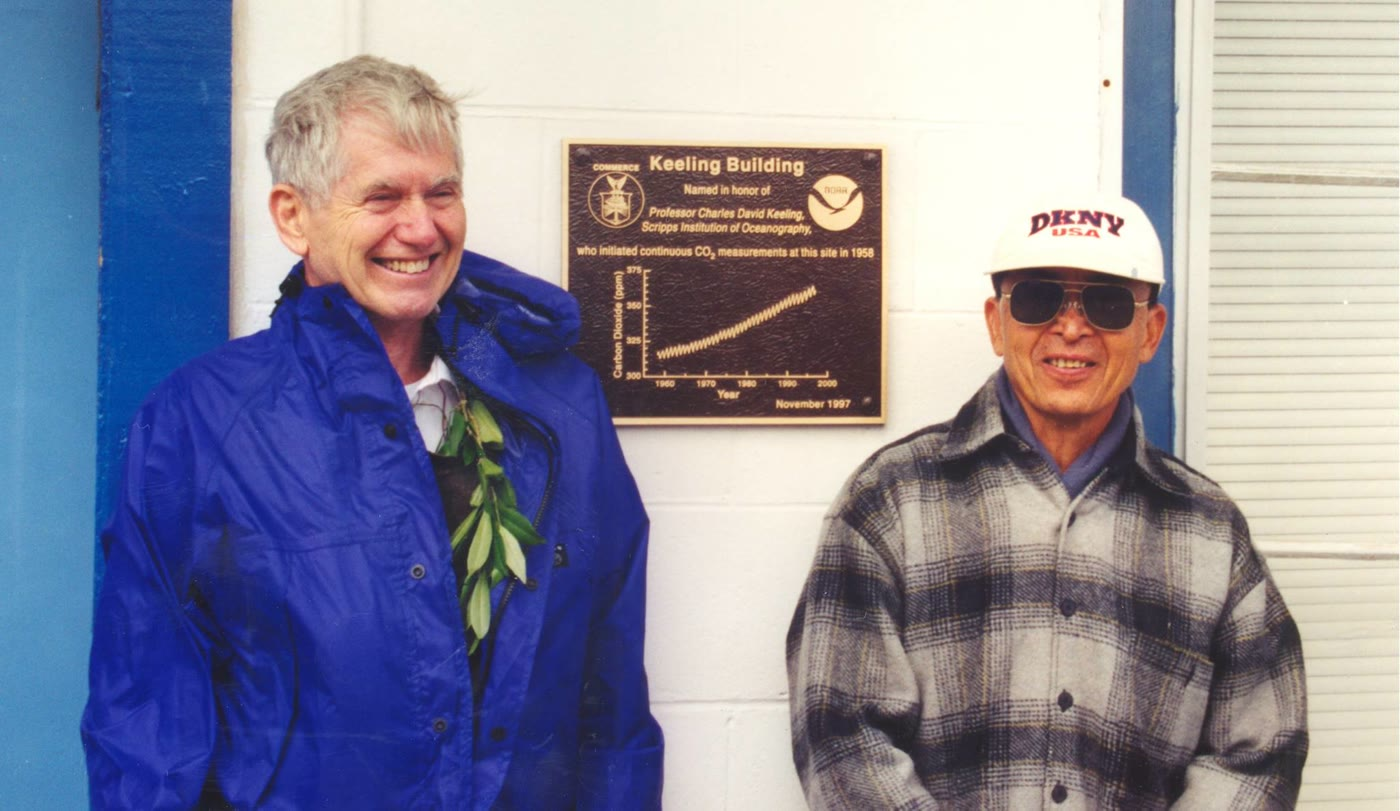
\includegraphics[width=0.62\linewidth]{images/book2/g12-noaa-keeling-chin-1997.jpg}

{\small Charles David Keeling (a la izquierda) y John Chin en el observatorio de
Mauna Loa en 1997, junto a la placa que da a un edificio el nombre de Keeling.
Fotografía: John Miller, NOAA (dominio público).}
\end{center}
\end{history}

\section{Ejercicios}

\begin{exercise}[$\star$]\label{exo:g12:climate-change:1}
¿Qué es el \omterm{def:g12:climate-change:forcing}{forzamiento radiativo} de un cambio en el sistema climático? ¿En qué
unidad se mide, y qué significa su signo?
\end{exercise}

\begin{exercise}[$\star$]\label{exo:g12:climate-change:2}
¿En qué mes del año es máxima la concentración de dióxido de carbono en Mauna Loa,
y en cuál es mínima? Explica la oscilación anual.
\end{exercise}

\begin{exercise}[$\star$]\label{exo:g12:climate-change:3}
En el vocabulario de las evaluaciones, ¿qué probabilidad significa \emph{muy
probable}? ¿Y \emph{probable}? ¿Qué significa un intervalo escrito
$[0.95 \text{ a } 1.20]$?
\end{exercise}

\begin{exercise}[$\star$]\label{exo:g12:climate-change:4}
De la energía adicional que el sistema climático ha ganado en las últimas décadas,
¿qué proporción fue al océano? ¿Por qué explica esto que el nivel del mar suba
incluso sin que se funda hielo?
\end{exercise}

\begin{exercise}[$\star$]\label{exo:g12:climate-change:5}
Da dos \omterm{def:g12:climate-change:feedback}{retroalimentaciones} climáticas positivas y la respuesta negativa que limita
el calentamiento. Explica cada una en una frase.
\end{exercise}

\begin{exercise}[$\star\star$]\label{exo:g12:climate-change:6}
La concentración media anual de dióxido de carbono en Mauna Loa fue de
\qty{315.98}{ppm} en 1959 y de \qty{427.35}{ppm} en 2025. ¿Cuántos ppm
aumentó, y en qué porcentaje? ¿Cuál fue el crecimiento medio por
año en todo el periodo?
\end{exercise}

\begin{exercise}[$\star\star$]\label{exo:g12:climate-change:7}
Usa la ley logarítmica del capítulo, con $F_{2\times} =
\qty{3.93}{W/m^2}$ y $C_0 = \qty{278}{ppm}$, para calcular el \omterm{def:g12:climate-change:forcing}{forzamiento} del
dióxido de carbono a \qty{427.35}{ppm}, la media anual de 2025.
\end{exercise}

\begin{exercise}[$\star\star$]\label{exo:g12:climate-change:8}
A \qty{3.7}{mm} al año, el ritmo de 2006--2018, ¿cuánto subiría el nivel del mar
en 30 años? ¿Cuántas veces más rápido es este ritmo que el de
1901--1971, \qty{1.3}{mm} al año?
\end{exercise}

\begin{exercise}[$\star\star$]\label{exo:g12:climate-change:9}
Con $\Delta T = F/\lambda$ y $\lambda = \qty{1.16}{W.m^{-2}.\degreeCelsius^{-1}}$,
calcula el calentamiento de equilibrio que produciría el \omterm{def:g12:climate-change:forcing}{forzamiento} humano total de 2019,
\qty{2.72}{W/m^2}. El calentamiento observado de origen humano es de solo
unos \qty{1.07}{\degreeCelsius}. Da la razón principal de la diferencia.
\end{exercise}

\begin{exercise}[$\star\star$]\label{exo:g12:climate-change:10}
El Sol y los volcanes cambiaron la temperatura global entre 1850--1900 y
2010--2019 de $-0.1$ a $+\qty{0.1}{\degreeCelsius}$, mientras que el calentamiento
observado fue de unos \qty{1.06}{\degreeCelsius}. ¿Qué puedes concluir? ¿Qué
otra causa natural hay que descartar también, y qué dice de ella la
evaluación?
\end{exercise}

\begin{exercise}[$\star\star$]\label{exo:g12:climate-change:11}
Con la tabla de proyecciones, ¿en qué \omterm{def:g12:climate-change:scenario}{escenarios} es muy probable que el calentamiento de
2081--2100 se quede por debajo de \qty{2}{\degreeCelsius}? ¿En cuáles es
muy probable que supere \qty{2}{\degreeCelsius}?
\end{exercise}

\begin{exercise}[$\star\star\star$]\label{exo:g12:climate-change:12}
Los aerosoles produjeron un \omterm{def:g12:climate-change:forcing}{forzamiento} de unos $-0.22$ y $\qty{-0.84}{W/m^2}$
(a través de la luz solar y a través de las nubes). Si se eliminaran todos los aerosoles del
aire y todo lo demás siguiera como en 2019, ¿cuánto valdría el \omterm{def:g12:climate-change:forcing}{forzamiento}
humano total? ¿Cuánto aumentaría el calentamiento de equilibrio, con
$\lambda = \qty{1.16}{W.m^{-2}.\degreeCelsius^{-1}}$?
\end{exercise}

\begin{exercise}[$\star\star\star$]\label{exo:g12:climate-change:13}
Demuestra, a partir de la ley logarítmica, que pasar de \qty{278}{ppm} a
\qty{556}{ppm} y pasar de \qty{556}{ppm} a \qty{1112}{ppm} añaden el mismo
\omterm{def:g12:climate-change:forcing}{forzamiento}. ¿Cuál es el \omterm{def:g12:climate-change:forcing}{forzamiento} total a \qty{1112}{ppm}?
\end{exercise}

\begin{exercise}[$\star\star\star$]\label{exo:g12:climate-change:14}
Deriva la ley logarítmica respecto a $C$. ¿Cuánto \omterm{def:g12:climate-change:forcing}{forzamiento} añade
un ppm más de dióxido de carbono a \qty{280}{ppm}, y cuánto a
\qty{420}{ppm}? Comenta.
\end{exercise}

\begin{exercise}[$\star\star\star$]\label{exo:g12:climate-change:15}
Sin ninguna \omterm{def:g12:climate-change:feedback}{retroalimentación} salvo la radiación adicional hacia el espacio,
$\lambda_0 = \qty{3.22}{W.m^{-2}.\degreeCelsius^{-1}}$. Calcula el calentamiento
para una duplicación del dióxido de carbono ($F_{2\times} = \qty{3.93}{W/m^2}$) con
$\lambda_0$, y luego con $\lambda = \qty{1.16}{W.m^{-2}.\degreeCelsius^{-1}}$. ¿Por
qué factor amplifican el calentamiento las \omterm{def:g12:climate-change:feedback}{retroalimentaciones}?
\end{exercise}

\section{Problema: la curva de Keeling en cifras}

\begin{problem}[{Problema de fin de semana --- de la respiración anual de la
vegetación al año en que se alcanzaría una duplicación}]
\label{pb:g12:climate-change:1}
% ledger: data:co2-mlo (annual means 1960 316.91, 1970 325.68, 2015 401.01,
% 2025 427.35; seasonal departures May +3.37, September -3.51, means of
% 2015-2024; all from figdata/grade-12/climate_records.py), noaa:mlo-site,
% ipcc:erf-2xco2, ipcc:ecs, ipcc:feedbacks, ipcc:co2-2myr
Una estudiante descarga el registro de Mauna Loa y lo trabaja con una
hoja de cálculo. En 2015--2024, la concentración mensual está en promedio
\qty{3.37}{ppm} por encima de la tendencia suavizada en mayo y \qty{3.51}{ppm} por debajo
en septiembre. Las medias anuales son \qty{316.91}{ppm} en 1960,
\qty{325.68}{ppm} en 1970, \qty{401.01}{ppm} en 2015 y \qty{427.35}{ppm}
en 2025. La concentración de 1750 era de \qty{278}{ppm}. Usa la ley logarítmica
con $F_{2\times} = \qty{3.93}{W/m^2}$.

\medskip
\noindent\textbf{Parte I --- La respiración de la vegetación.}
\begin{enumerate}
  \item ¿Cuál es la amplitud entre el máximo y el mínimo del ciclo anual?
  \item Explica por qué la concentración es máxima en mayo y mínima en
        septiembre.
  \item El ciclo es mucho más débil en el aire del hemisferio sur.
        Propón una explicación.
  \item ¿Por qué se construyó el observatorio a \qty{3397}{m} de altitud, sobre un volcán en
        medio del Pacífico?
\end{enumerate}

\medskip
\noindent\textbf{Parte II --- La tendencia.}
\begin{enumerate}[resume]
  \item Calcula el crecimiento medio, en ppm al año, en 1960--1970.
  \item Calcúlalo en 2015--2025.
  \item ¿Por qué factor ha aumentado el ritmo de crecimiento?
  \item ¿En qué porcentaje subió la concentración entre 1750 y
        2025?
  \item Los \omterm{def:g12:past-climates:ice-core}{testigos de hielo} nunca muestran más de unos \qty{300}{ppm} en los
        últimos 800\,000 años. ¿En cuántos ppm supera el valor de 2025
        esta cifra?
\end{enumerate}

\medskip
\noindent\textbf{Parte III --- El forzamiento.}
\begin{enumerate}[resume]
  \item Calcula el \omterm{def:g12:climate-change:forcing}{forzamiento} del dióxido de carbono en 2025.
  \item Calcúlalo en 1960, y el aumento del \omterm{def:g12:climate-change:forcing}{forzamiento} entre 1960
        y 2025.
  \item ¿Qué concentración añadiría \qty{1}{W/m^2} al \omterm{def:g12:climate-change:forcing}{forzamiento} de 2025?
  \item Al ritmo de crecimiento de 2015--2025, ¿cuántos años tardaría en alcanzarse?
\end{enumerate}

\medskip
\noindent\textbf{Parte IV --- La duplicación.}
\begin{enumerate}[resume]
  \item ¿Cuál es la concentración de una duplicación del valor de 1750? ¿Qué
        \omterm{def:g12:climate-change:forcing}{forzamiento} produce?
  \item Con la mejor estimación de la \omterm{def:g12:climate-change:ecs}{sensibilidad climática de equilibrio},
        ¿qué calentamiento de equilibrio causaría? Da el intervalo probable.
  \item ¿Qué parámetro de \omterm{def:g12:climate-change:feedback}{retroalimentación} $\lambda$ implica una sensibilidad de
        \qty{3}{\degreeCelsius}? Compáralo con el valor
        \qty{1.16}{W.m^{-2}.\degreeCelsius^{-1}} obtenido sumando las
        \omterm{def:g12:climate-change:feedback}{retroalimentaciones}.
  \item ¿Por qué la superficie no alcanzaría este calentamiento el mismo día en que
        se alcance la duplicación?
  \item ¿Por qué un cálculo que simplemente prolonga el ritmo de crecimiento actual es un
        \omterm{def:g12:climate-change:scenario}{escenario}, y no una \omterm{def:g12:climate-change:scenario}{proyección} del tipo que hacen las evaluaciones?
  \item Si el ritmo de crecimiento de 2015--2025 se mantuviera, ¿en qué año
        se alcanzaría la duplicación de la concentración de 1750?
\end{enumerate}
\end{problem}
